\documentclass{tufte-handout}
\usepackage{graphicx}
\usepackage{enumitem}

\title{Tic Tac Toe Overview}
\author{James Richey}

% \geometry{showframe}

\begin{document}


\maketitle


% Concept art that shows the visual style of the game is shown in
% the right margin.
\begin{marginfigure}
  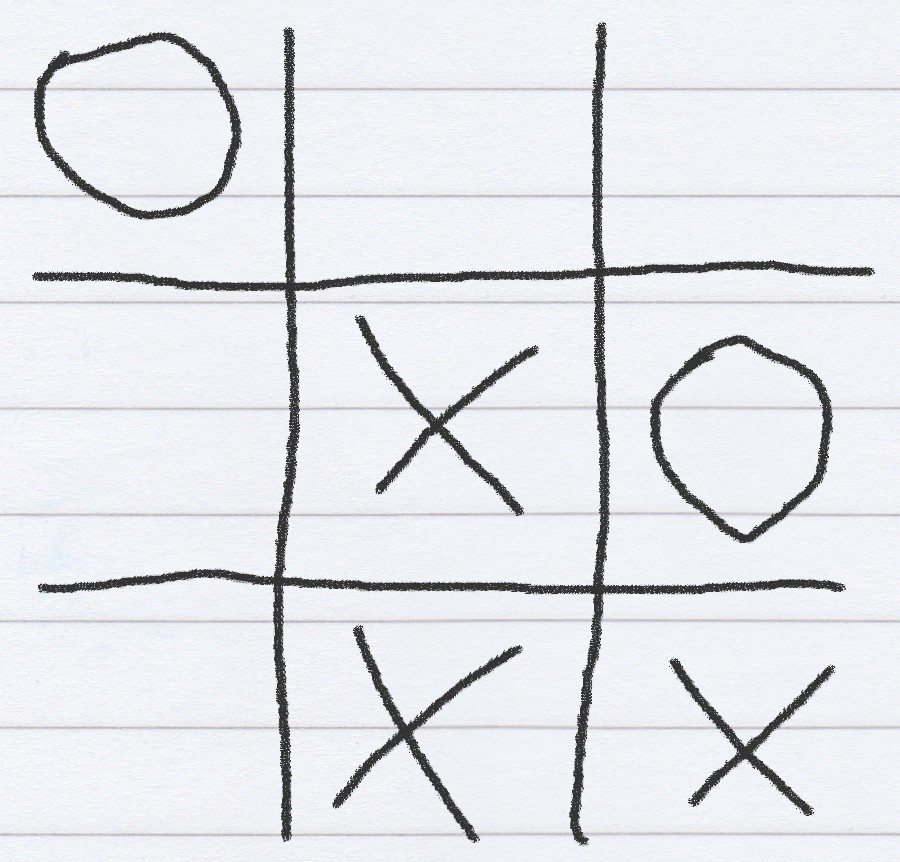
\includegraphics[width=\linewidth]{img/concept-art/paper}
  Notebook paper
\end{marginfigure}

\begin{marginfigure}
  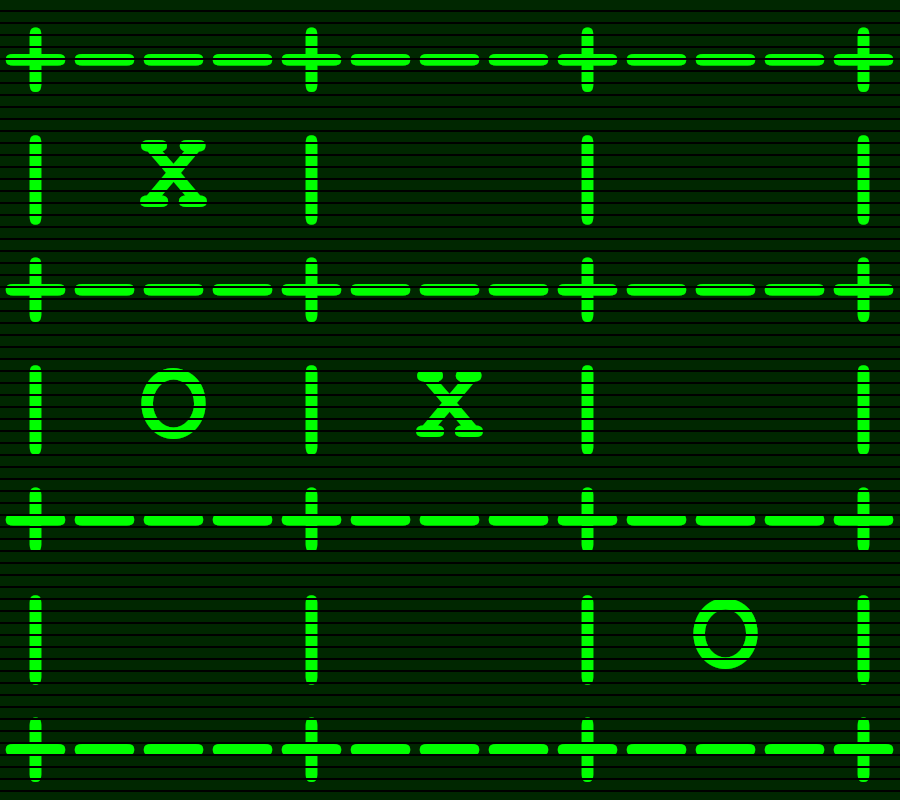
\includegraphics[width=\linewidth]{img/concept-art/computer}
  Early computer
\end{marginfigure}

\begin{marginfigure}
  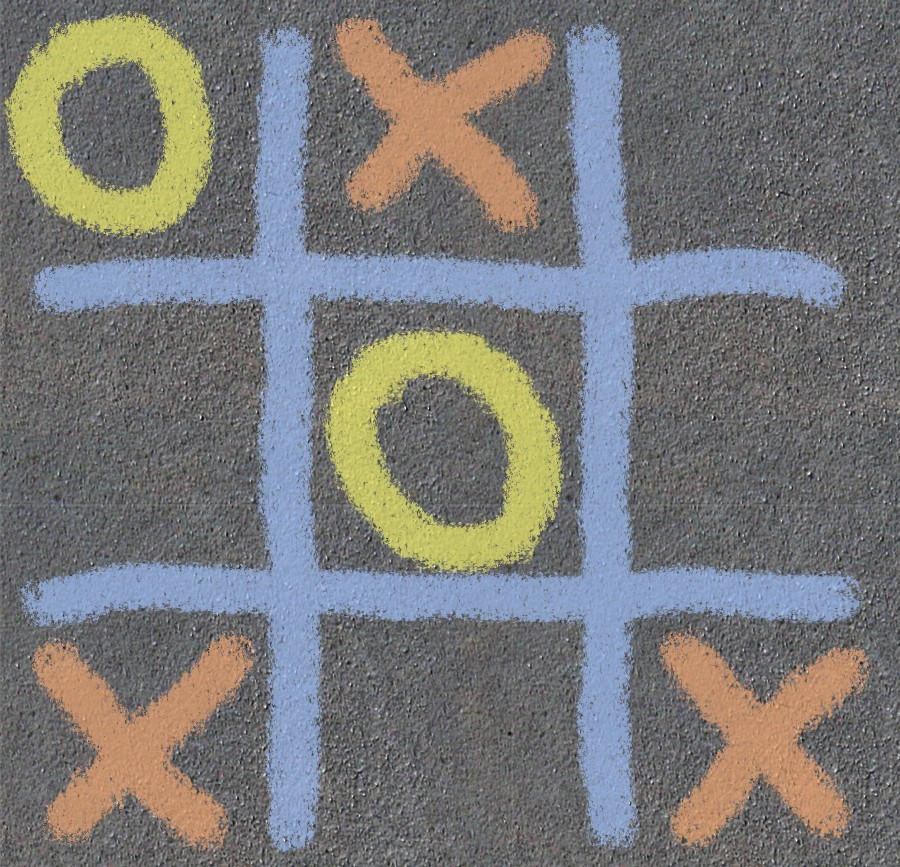
\includegraphics[width=\linewidth]{img/concept-art/sidewalk}
  Sidewalk
\end{marginfigure}

\begin{marginfigure}
  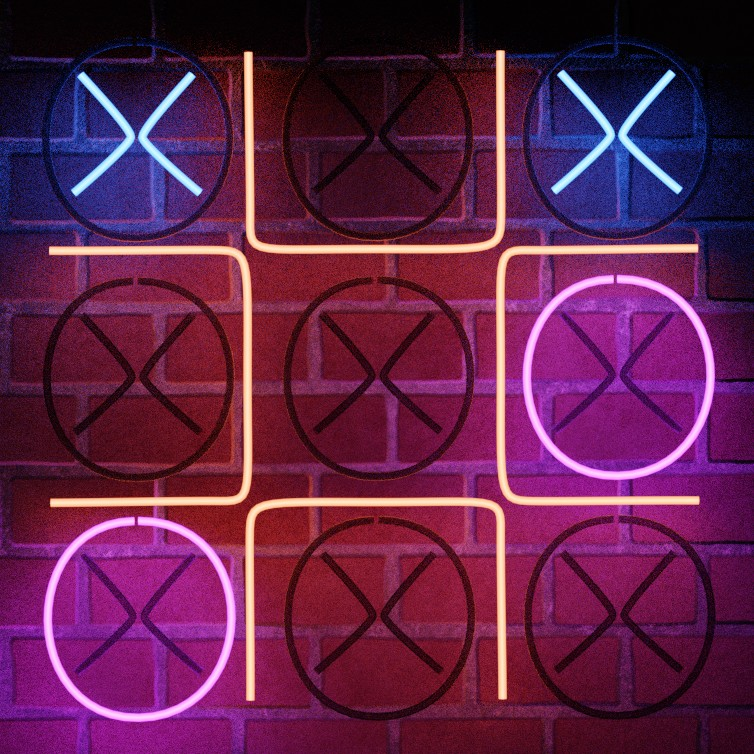
\includegraphics[width=\linewidth]{img/concept-art/neon}
  Neon lights
\end{marginfigure}


\begin{abstract}
  \begin{itemize}[noitemsep,label=]
    \item A casual game for all ages
    \item Windows, Linux, and Mac
    \item Coming Summer 2020
  \end{itemize}
\end{abstract}


\section{Game Summary}
Tic Tac Toe is an unique take on a classic game. Players battle the computer or
each other in a variety of stunning environments. Each environment tells part of
the story of Tic Tac Toe from the past, present, and future. Each environment
has a strong visual theme and complementary soundtrack.


\section{Game Outline}
Tic Tac Toe is a game of strategy where two players, X and O, take turns placing
their mark in a $3\times3$ gird. The first player to get three marks in a row,
column, or diagonal wins the game. The game can also end in a draw, known as a
``cat's game,'' if all the free spaces are exhausted.

Players alternate who gets to make the first move in the game. Additionally,
each game takes place in a different environment keeping players engaged.


\section{Unique Selling Points}
\begin{itemize}[noitemsep]
  \item {
    Over 20 beautiful environments including classic paper-and-pencil, modern
    computer screens, and futuristic cyber punk.
  }
  \item Amazing soundtrack for a fully immersive experience.
  \item Challenging AI that is ready to counter any strategy.
  \item Battle your friends with local multiplayer.
  \item Free, open source, and no annoying advertisements.
\end{itemize}


\section{Similar Games}
\begin{itemize}[noitemsep]
  \item OXO
  \item Tic Tac Toe (2004) by James Richey
  \item Connect 4
\end{itemize}


\end{document}
